\section{Introduction}

A \textbf{linear interpolator} is a digital circuit that implements the following function:

\begin{displaymath}
    y(nT+uT) = (y_{n+1} - y_n)u + y_n \qquad u=\frac{k}{L}, k \in \{0,1,...,L-1\}
\end{displaymath}

In general, given \textbf{two consecutive input signals} sampled every $T$, the interpolator generates $L$ \textbf{output signals}, with a period of $\frac{T}{L}$ (for this reason $L$ is defined \textbf{factor of interpolation}). If the two input signals represent two points on a cartesian plane, the output signals lie on the line that connects the two inputs.

\subsection{Design Specifications}

The interpolator shall have the following characteristics:

\begin{itemize}
    \item \textbf{Input} and \textbf{output} are represented by 16 bit, so they can assume any integer values between 0 and 65535.
    \item The input signals have a \textbf{sampling period} of $T$, so the circuit will receive every $T$ a new signal.
    \item The factor of interpolation is fixed to $L=4$. So the \textbf{period} with which \textbf{output signals} have to be produced is $\frac{T}{4}$.
\end{itemize}

Moreover the structure of the circuit's \textbf{I/O ports} have to be the following:

\begin{figure}[H]
    \centering
    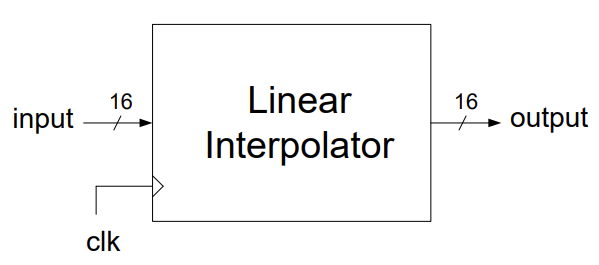
\includegraphics[width=0.5\textwidth]{img/IOPorts.png}
    \caption{Circuit's I/O Ports}
    \label{fig:IOPorts}
\end{figure}

\subsection{Useful Symbols}

The following \textbf{symbol} will be used to identify the signals:

\begin{itemize}
    \item $y_{n+1}$, is the last received signal.
    \item $y_n$, is the second last received signal.
    \item $OUT_i$, is one of the four output signals.
\end{itemize}